\DiaryEntry{Subband Coding}{2021-11-09}{Coding}

Working with signals in the temporal or spatial domain allowed us to use their correlation properties to develop techniques such as differential encoding and vector quantization. Working with signals in the frequency domain allowed us to use their spectral structure and develop transform coding approaches. In each case we stayed exclusively in one domain—either temporal and spatial or spectral.


In subband coding the signal is decomposed into frequency bands after which the temporal or spatial signal in each band can be separately encoded. This allows us to make use of the very different kinds of structures that exist in each band. The low frequency signals tend to be smoother allowing us to use sample to sample correlation if we wish. The high frequency signals tend to be sparse allowing us to use schemes more appropriate to sparse signals. Subband decomposition also permits the exploitation of both spectral and temporal limitations of human perception which can let us selectively ignore or discard components of the signal.


\subsection{Overview}

Subband coding uses the following structure.


\begin{figure}[H]
    \centering
    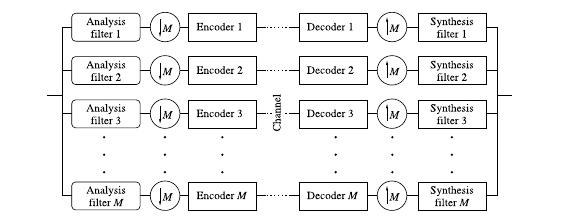
\includegraphics[scale=0.7]{images/2021-11-09-subband_01.png}
\end{figure}


\paragraph{Analysis.} The source output is passed through a bank of filters, called the analysis filter bank, which covers the range of frequencies that make up the source output. The passbands of the filters can be nonoverlapping or overlapping. The outputs of the filters are then subsampled; the filters are designed in such a way as to limit the bandwidth of the signals and therefore no information is lost due to subsampling. Of course, the filters need to be chosen accordingly.



\paragraph{Quantization and Coding.} Once the output of the filters has been subsampled, the output is encoded using one of several encod- ing schemes, including ADPCM, PCM, and vector quantization.

Along with the selection of the compression scheme, the allocation of bits between the subbands is an important design parameter. Different subbands contain differing amounts of information. Therefore, we need to allocate the available bits among the subbands according to some measure of the information content. There are a number of different ways we could distribute the available bits. 


\paragraph{Synthesis.} The quantized and coded coefficients are used to reconstruct a representation of the original signal at the decoder. First, the encoded samples from each subband are decoded at the receiver. These decoded values are then upsampled by inserting an appropriate number of $0$s between samples. Once the number of samples per second has been brought back to the original rate, the upsampled signals are passed through a bank of reconstruction filters. The outputs of the reconstruction filters are added to give the final reconstructed outputs.

\qed

We can see that the basic subband system is simple. The three major components of this system are the analysis and synthesis filters, the bit allocation scheme, and the encoding scheme. A substantial amount of research has focused on each of these components. Various filter bank structures have been studied in order to find filters that are simple to implement and provide good separation between the frequency bands.

The separation of the source output according to frequency also opens up the possibility for innovative ways to use compression algorithms. The decomposition of the source output in this manner provides inputs for the compression algorithms, each of which has more clearly defined characteristics than the original source output. We can use these characteristics to select separate compression schemes appropriate to each of the different inputs.

Human perception of audio and video inputs is frequency dependent. We can use this fact to design our compression schemes so that the frequency bands that are most important to perception are recon- structed most accurately. Whatever distortion there has to be is introduced in the frequency bands to which humans are least sensitive. We describe some applications to the coding of speech, audio, and images later in this chapter.


\subsection{Filterbanks}

Suppose we have a sequence $x_0, x_1, x_2 , \ldots$. We can divide this sequence into two subsequences: $x_0, x_2, x_4, \ldots$ and $x_1, x_3, x_5, \ldots$ using the scheme shown in the Figure below. This subsampling process is called \emph{downsampling} or \emph{decimation}.

\begin{figure}[H]
    \centering
    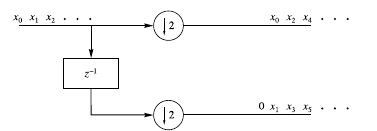
\includegraphics[scale=0.6]{images/2021-11-09-subband_02.png}
\end{figure}



The original sequence can be recovered from the two downsampled sequences by inserting $0$s between consecutive samples of the subsequences, delaying the top branch by one sample and adding the two together. Adding $0$s between consecutive samples is called upsampling. The reconstruction process is shown in the following Figure.

\begin{figure}[H]
    \centering
    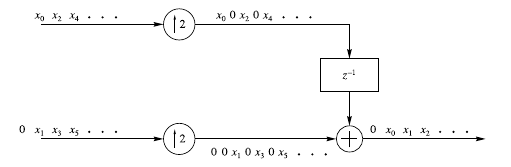
\includegraphics[scale=0.6]{images/2021-11-09-subband_03.png}
\end{figure}


A generalized filterbank system is shown in the following Figure: The source sequence $x[n]$ is fed into two \emph{analysis} filters $H_1(z)$ and $H_2(z)$, resulting into the signals $y_1[n]$ and $y_2[n]$. The signals are downsampled resulting in signals $v_1[n], v_2[n]$. Then the signals are encoding / decoded and upsampled, resulting in $u_1[n], u_2[n]$. After filtering with \emph{synthesis} $F_1(z), F_2(z)$, the signals are added, yielding the filterbank output signal $y[n]$.

\begin{figure}[H]
    \centering
    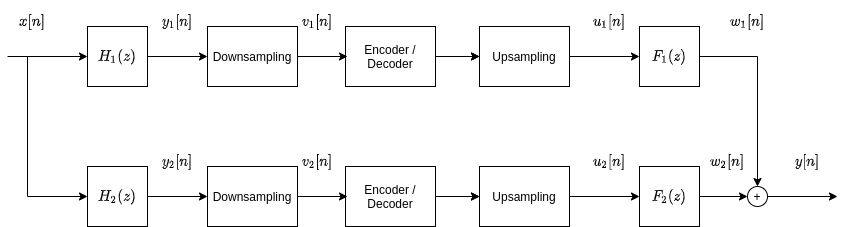
\includegraphics[scale=0.5]{images/2021-11-09-subband_04.png}
\end{figure}


We next investigate how up/down-sampling operates in the frequency domain.


\paragraph{Upsampling.} A signal $x[n]$ is upsampled by a factor $2$, yielding an output sequence $y[n]$ according to

\bee
y[n] = \begin{cases} x[n/2] & \text{ for $n$ even} \\ 0 & \text{otherwise} \end{cases}
\eee

Between every signal point a zero is inserted and therefore no information is lost. The z-transform of the output is given by

\bee
Y(z) = \sum_n y[n] z^{-n} = \sum_{n \text{even}} y[n] z^{-n} = \sum_{k} y[2k] z^{-2k} = \sum_{k} x[k] z^{-2k} = X(z^2)
\eee

For the DFT, we obtain

\bee
Y(e^{j \omega}) = X(e^{j 2 \omega})
\eee

which corresponds to a compression of the spectrum. This is shown in the following Figure.

\begin{figure}[H]
    \centering
    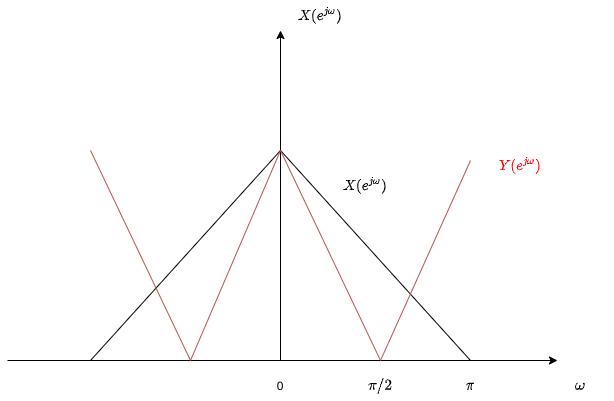
\includegraphics[scale=0.5]{images/2021-11-09-subband_05.png}
\end{figure}


\paragraph{Downsampling.} A signal $x[n]$ is downsampled by a factor of $2$, yielding a signal $y[n]$ given by

\bee
y[n] = x[2n]
\eee

Every second signal point is removed, therefore information is lost. The z-transform of the output signal can be shown to equal (proof omitted)

\bee
Y(z) = \frac{1}{2} X(z^{1/2}) + \frac{1}{2} X(-z^{1/2})
\eee

and the spectrum is

\bee
Y(e^{j \omega}) = \frac{1}{2} \left( X(e^{j \omega/2}) + X(e^{j(\omega - 2\pi)/2} \right)
\eee

This is shown in the following Figure (the factor two is omitted). In the upper part of the Figure the bandwidth of the signal to be downsampled is $\pi/2$, therefore the spectrum of the downsampled signal reaches up to $\pi$ and no information is lost.

In the lower part, the bandwith of $x[n]$ is larger than $\pi/2$ and the downsampling introduces aliasing; i.e. information is lost.

\begin{figure}[H]
    \centering
    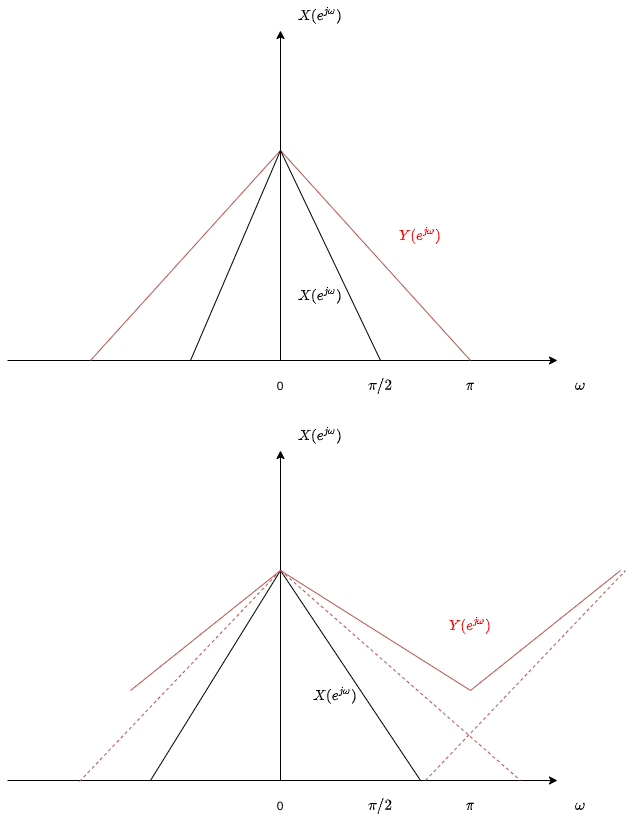
\includegraphics[scale=0.5]{images/2021-11-09-subband_06.png}
\end{figure}



\paragraph{Combination of Filter and Up-/Downsampler.} Next we consider a filter combined with an up- or downsampler as shown in the following Figure. If a signal is downsampled by a factor $M$ and filtered afterwards by a filter $F(z)$, we can replace it with a structure of a filter $F(z^m)$ followed by the downsampler of factor $M$.

A similar correspondence is also available for a filter follwed by an upsampler (by a factor of $L$): The equivaent structure is the upsampler (factor $L$) follwed by the filter $F(z^L)$. 


\begin{figure}[H]
    \centering
    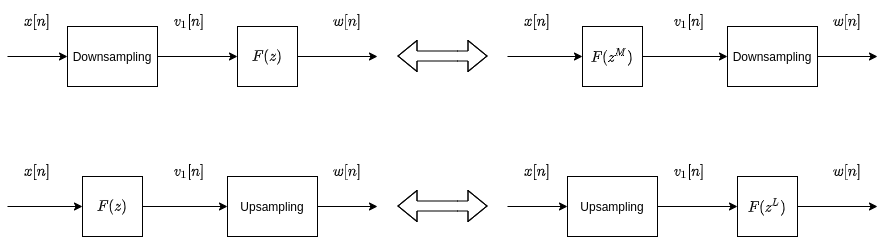
\includegraphics[scale=0.45]{images/2021-11-09-subband_06a.png}
\end{figure}

These identities can be used to obtain the input-output relation from a system consisting of filters, up-, and downsamplers in various combinations.

\qed

Now consider a combined downsampling / upsampling system as shown below. This corresponds to one part of the filter bank described previously.


\begin{figure}[H]
    \centering
    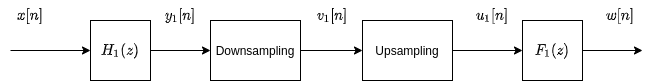
\includegraphics[scale=0.5]{images/2021-11-09-subband_07.png}
\end{figure}

Downsampling $y_1[n]$ throw away information; in order to avoid this, the signal bandwith must be less than $\pi/2$. One choice is that  $y_1[n]$ is a low-pass signal with bandwidth less than $\pi/2$. Either the input signal $x[n]$ is already such a low-pass signal (in this case, we can omit the filter $H_1(z)$) or we filter $x[n]$ with $H_1(z)$ to obtain a suitable low-pass signal. Downsampling spreads the spectrum by a factor of two, upsampling compresses the spectrum and introduces spectrum components above $\pi/2$. The output filter $F_1(z)$ can remove these unwanted frequency components, yielding $w[n]$.

The spectra of the various signals are shown in the following Figure. The spectrum $X(e^{j\omega})$ (shown in red) has bandwidth larger $\pi/2$. It is filtered by an ideal lowpass $H_1(z)$; i.e. everything is cut above $\pi/2$. Downsampling yields $V_1$ which has a bandwidth of $\pi$. Upsampling compresses the spectrum, yielding $U_1$. The filter $F_1$ removes frequency components above $\pi/2$ and we have reconstructed the signal $y_1[n]$.

\begin{figure}[H]
    \centering
    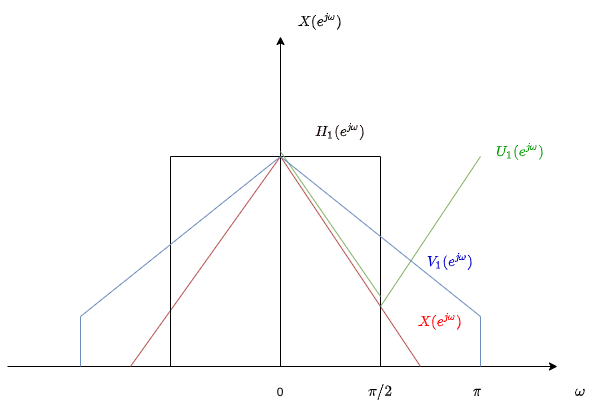
\includegraphics[scale=0.5]{images/2021-11-09-subband_08.png}
\end{figure}

However, this is not the only possible setup; we could also filter the input signal with a highpass filter $H_1$, downsample and upsample. The signal $w_1[n]$ will now be spread acorss the whole spectrum and have alias components at frequencies below $\pi/2$. The filter $F_1$ can remove these alias components ($F_1$ should be a highpass filter to this end).

In the next Section, we will derive the input-output relation for the filterbank; sneaking forward a bit, we have the following input-output relation for the system under consideration

\bee
Y(z) &= \frac{1}{2} H_1(z) F_1(z) X(z) + \frac{1}{2} H_1(-z) F_1(z) X(-z)
\eee

We see that there is contribution from $X(z)$ and one from $X(-z)$; the second part represents the aliasing introduced by the upsampling. Note that $H(-z) = H(-e^{j \omega}) = H(e^{j \pi} e^{j \omega}) = H(e^{j(\omega + \pi)})$; this corresponds to a spectrum centered at $\pi$ and is therefore the aliasing term.

If we choose $H_1$ and $F_1$ as perfect lowpass filters with bandwith $\pi/2$, then $H_1(-z)$ becomes a highpass with bandwidth $\pi/2$ and multiplying with the ideal lowpass $F_1$ yields $0$ for all frequencies. We therefore have

\bee
Y(e^{j \omega}) = \begin{cases} \frac{1}{2} H_1(e^{j \omega}) F_1(e^{j \omega})=1 & \omega < \pi/2 \\ 0 & \omega > \pi/2 \end{cases}

\qed


Coming back to our filter bank, we see that we have two upsampling / downsampling paths. In order to get perfect reconstruction, we have 4 filters (the two analysis filters $H_1(z), H_2(z)$ and the two synthesis filters $F_1(z), F_2(z)$) as ``design space'' so that $y[n] = x[n]$.


\subsection*{Filterbank Input-Output Relation}

We will derive the relation between the input $X(z)$ and the output $Y(z)$ in terms of the 4 filters $H_1, H_2, F_1, F_2$. We have

\bee
Y(Z) = U_1(z) F_1(Z) + U_2(z) F_2(z)
\eee

The signal $U_i(z)$ are obtained by upsampling $V_i(z)$, therefore $U_i(z) = V_i(z^2)$ and we have

\bee
Y(Z) = V_1(z^2) F_1(Z) + V_2(z^2) F_2(z)
\eee

The signals $V_i(z)$ are obtained from downsampling $Y_i(z)$ and we have the following relation

\bee
V_i(z) = \frac{1}{2} Y_i(z^{1/2}) + \frac{1}{2} Y_i(-z^{1/2})
\eee

and $Y_i(z) = X(z) H_i(z)$.

Let's consider the effect of down- and upsampling,

\bee
U_i(z) = V_i(z^2) = \frac{1}{2} Y_i(z) + \frac{1}{2} Y_i(-z) = \frac{1}{2} X(z) H_i(z) + \frac{1}{2} X(-z) H_i(-z)
\eee

and we finally arrive at

\begin{align*}
Y(z) &= \frac{1}{2} \left[  X(z) H_1(z) + X(-z) H_1(-z) \right]  F_1(Z) + \frac{1}{2} \left[ X(z) H_2(z) +  X(-z) H_2(-z) \right] F_2(z) \\
= &\frac{1}{2} \left[ H_1(z) F_1(z) + H_2(z) F_2(z) \right] X(z) + \\
&+ \frac{1}{2} \left[ H_1(-z) F_1(z) + H_2(-z) F_2(z) \right] X(-z)
\end{align*}

We have separated the terms into one for $X(z)$ and one "aliasing" term for $X(-z)$. For perfect reconstruction, we want to have

\bee
Y(z) = c X(z) z^{-n_0}
\eee

i.e. we want a delayed and scaled version of the input at the output. This can be achieved by the following two conditions

\begin{align*}
H_1(z) F_1(z) + H_2(z) F_2(z) &= c z^{-n_0} \\
H_1(-z) F_1(z) + H_2(-z) F_2(z) &= 0
\end{align*}


\subsection*{Quadrature Mirror Filter Banks}




%%% Local Variables:
%%% mode: latex
%%% TeX-master: "journal"
%%% End:
